\documentclass[../../main.tex]{subfiles}
\begin{document}

$xy$ 平面上の $y \geqq x^2$ で表される領域を $D$ とする．
$D$ に含まれる1辺の長さ $t$ の正方形で，各辺が座標軸と平行または $45^\circ$ の角をなすものをすべて考える．

このとき，これらの正方形の中心の $y$ 座標の最小値を $t$ の関数として表し，そのグラフをかけ．

\begin{figure}[htbp]
  \centering
  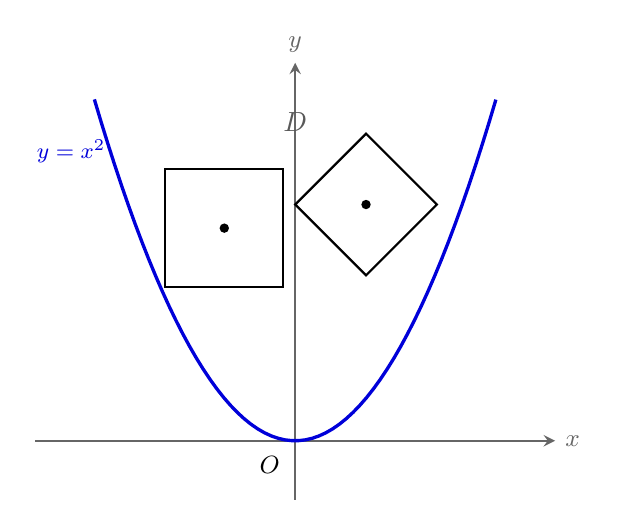
\begin{tikzpicture}[scale=1.5, >=stealth, every node/.style={font=\small}]
    % 座標軸
    \draw[->, thick, gray!80!black] (-2.2, 0) -- (2.2, 0) node[right] {$x$};
    \draw[->, thick, gray!80!black] (0, -0.5) -- (0, 3.2) node[above] {$y$};
    \node[below left=2pt] at (0, 0) {$O$};

    % 放物線 y = x^2
    \draw[very thick, blue!85!black, domain=-1.7:1.7, samples=60] plot (\x, {\x*\x});
    \node[blue!85!black, above left=1pt, font=\footnotesize] at (-1.5, 2.25) {$y=x^2$};
    \node[gray!70!black, font=\bfseries] at (0, 2.7) {$D$};

    % 座標軸に平行な正方形 (D の内部)
    % x \in [-1.1, -0.1], y \in [1.3, 2.3], 中心 (-0.6, 1.8)
    \draw[thick] (-1.1, 1.3) rectangle (-0.1, 2.3);
    \node[circle, fill, inner sep=1.2pt] at (-0.6, 1.8) {};

    % 45° 傾いた正方形 (D の内部)
    % 中心 (0.6, 2.0), 半対角線 0.6
    \begin{scope}[shift={(0.6, 2.0)}, rotate=45]
      \draw[thick] (-0.424, -0.424) rectangle (0.424, 0.424);
      \node[circle, fill, inner sep=1.2pt] at (0, 0) {};
    \end{scope}
  \end{tikzpicture}
  \caption{問題の図}
  \label{fig:problem}
\end{figure}

\end{document}
